\chapter{Discesa Ricorsiva sulla Sintassi Astratta}
  \label{chap:recursive_descent}
%
\begin{center}
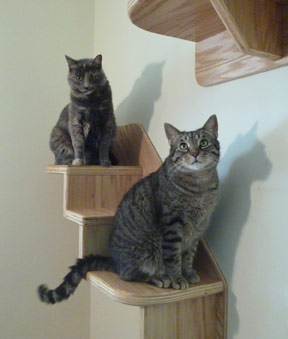
\includegraphics[width=6cm]{paw.jpg}
\end{center}
%
In questo capitolo discutiamo l'implentazione di algoritmi che
scendono ricorsivamente sull'albero di sintassi astratta che l'analizzatore
sintattico ha generato a partire da un file sorgente. Tali algoritmi
hanno le funzioni pi\`u svariate, da una semplice raccolta di dati statistici
sul codice alla verifica dell'uso corretto degli identificatori,
dalla determinazione del \emph{codice morto}, \cioe di porzioni di codice
che sicuramente non vengono raggiunte dal flusso di controllo e possono
quindi essere eliminate,
alla rappresentazione grafica della sintassi astratta, fino
al type-checking del codice (a cui dedicheremo,
per la sua complessit\`a, l'intero Capitolo~\ref{chap:semantical})
o addirittura alla generazione del codice intermedio,
descritta nel Capitolo~\ref{chap:translate}.
L'implementazione di questi algoritmi tramite discesa ricorsiva
sulla sintassi astratta, piuttosto
che tramite azioni semantiche (Capitolo~\ref{chap:syntactical}),
permette di sfruttare la gerarchia delle classi di sintassi astratta per
Kitten descritta nel Capitolo~\ref{chap:syntactical}, definendo l'algoritmo
ricorsivo tramite un metodo virtuale ricorsivo delle classi di sintassi
astratta.

Si consideri per esempio la grammatica in Figura~\ref{fig:grammar_lists}.
Supponiamo di voler contare
il numero di \texttt{a} e il numero di \texttt{b} di ciascun file sorgente
che rispetta le regole espresse dalla grammatica. Abbiamo gi\`a risolto questo
problema in Figura~\ref{fig:grammar_lists_decoration} tramite azioni
semantiche. Ma possiamo fare la stessa cosa generando la sintassi astratta
tramite le regole in Figura~\ref{fig:grammar_lists_abstract_syntax} e
aggiungendo alle classi di sintassi astratta un metodo
\texttt{count()} che conta il numero di \texttt{a} o di \texttt{b}
contenute nella sintassi concreta rappresentata dall'albero di sintassi
astratta. Il codice \`e mostrato nella Figura~\ref{fig:grammar_lists_count}.
Le classi \texttt{AbstractA}, \texttt{EmptyA} e \texttt{OneA} sono
simili a quelle mostrate nella figura per \texttt{B}.
La classe \texttt{Pair} \`e la
stessa usata nella Sezione~\ref{sec:abstract_syntax} (una coppia di interi).
%
\begin{figure}[t]
\begin{verbatim}
     public abstract class AbstractB {
       public abstract int count();
     }

     public class EmptyB extends AbstractB {
       public int count() { return 0; }
     }

     public class OneB extends AbstractB {
       private final AbstractB l;
       public OneB(AbstractB l) { this.l = l; }
       public int count() { return 1 + l.count(); }
     }

     public class AB {
       private final AbstractA a;
       private final AbstractB b;
       public AB(AbstractA a, AbstractB b) { this.a = a; this.b = b; }
       public Pair count() {
         return new Pair(a.count(), b.count());
       }
     }
\end{verbatim}
\caption{Un metodo ricorsivo che conta il numero di \texttt{a} e di \texttt{b}
         nella sintassi astratta generata come in
         Figura~\ref{fig:grammar_lists_decoration}.}
  \label{fig:grammar_lists_count}
\end{figure}

Va subito osservato che in Figura~\ref{fig:grammar_lists_count} sono
definiti \emph{due} metodi \texttt{count()}. Il primo \`e quello
ricorsivo delle classi \texttt{EmptyB} e \texttt{OneB}; il secondo \`e quello
\emph{non ricorsivo} della classe \texttt{AB}. Esiste anche un metodo
\texttt{count()} ricorsivo dentro \texttt{EmptyA} e \texttt{OneA} che non
\`e mostrato in figura in quanto \`e simmetrico a quello in
\texttt{EmptyB} e \texttt{OneB}.
Il metodo \texttt{count()} di \texttt{EmptyB} e \texttt{OneB} \`e
\emph{a discesa ricorsiva sulla sintassi astratta} poich\'e la sua
chiamata scende ricorsivamente sui componenti della sintassi astratta fino
ad arrivare alle foglie, per le quali \`e definito un valore costante.
Si faccia attenzione al fatto che
il metodo virtuale \texttt{count()} \`e dichiarato
\texttt{abstract} nella superclasse astratta \texttt{AbstractB} e quindi
\emph{deve} essere implementato in ognuna delle sue sottoclassi.

Cosa abbiamo guadagnato rispetto all'uso di azioni semantiche come
in Figura~\ref{fig:grammar_lists_decoration}? In primo luogo abbiamo lasciato
l'analizzatore sintattico alla sua occupazione pi\`u specifica, \cioe
all'analisi sintattica, piuttosto che usarlo per funzioni a lui \emph{improprie}
tramite azioni semantiche, rispettando quindi il principio della separation
of concerns. In secondo luogo abbiamo \emph{concentrato}
delle funzioni della sintassi astratta nelle classi di sintassi astratta
stesse, sotto forma di codice Java ricorsivo, che pu\`o essere complesso
quanto vogliamo. In terzo luogo possiamo utilizzare la gerarchizzazione delle
classi di sintassi astratta (come quella discussa per Kitten nella
Sezione~\ref{sec:abstract_syntax_classes}) per definire i metodi virtuali
solo su alcune superclassi, lasciandoli ereditare a tutte le loro sottoclassi,
nei casi in cui essi non differissero da una sottoclasse all'altra.
Questo non \`e possibile tramite azioni semantiche che, anche quando sono
identiche per \piu produzioni della grammatica,
devono essere comunque duplicate per ognuna di esse.
Quest'ultimo aspetto sar\`a chiaro adesso considerando un esempio di
discesa ricorsiva sulla sintassi astratta di Kitten.
%
\section{Determinazione delle variabili che occorrono in un'espressione o comando}
  \label{sec:free_variables}
%
Espressioni e comandi Kitten possono contenere variabili.
Per esempio, le variabili che \emph{occorrono} (sono contenute)
nell'espressione Kitten \texttt{x + 3 * y} sono \texttt{x} e \texttt{y}.
Le variabili che occorrono nel comando Kitten
\texttt{x := 12 + a} sono \texttt{x} e \texttt{a}.
Ci proponiamo adesso di definire formalmente e poi di calcolare l'insieme delle
variabili che occorrono in un'espressione e poi l'insieme delle variabili che
occorrono in un comando.

Cominciamo con le espressioni (Figura~\ref{fig:expressions_hierarchy}).
Definiamo una funzione
\[
  \vars{\_}:\mathtt{Expression}\mapsto\wp(\mathtt{String})
\]
che mappa ciascuna espressione nell'insieme dei nomi delle variabili
che occorrono nell'espressioni. Alcuni casi della
definizione di questa funzione sono particolarmente semplici. Per esempio,
una variabile occorre in se stessa:
\begin{equation}\label{eq:vars_variable}
  \vars{\mathtt{Variable(name)}}=\{\mathtt{name}\}
\end{equation}
mentre i letterali non contengono variabili:
\begin{equation}\label{eq:vars_literal}
  \vars{\mathtt{Literal()}}=\emptyset~.
\end{equation}
Si noti che quest'ultima equazione definisce l'insieme delle variabili che
occorrono in ogni sottoclasse di \texttt{Literal} in
Figura~\ref{fig:expressions_hierarchy}, senza bisogno di ripetere l'equazione
per ogni sottoclasse.

Un po' \piu complesso \`e il caso del meno unario e della negazione logica che,
che contenendo ricorsivamente un'altra espressione, danno origine a una
definizione ricorsiva per $\vars{}$ (ma ben fondata perch\'e andiamo verso
strutture sintattiche sempre \piu piccole):
\[
  \vars{\mathtt{Minus(expression)}}=\vars{\mathtt{Not(expression)}}
    =\vars{\mathtt{expression}}~.
\]
Un cast e la creazione di un array contengono sia un tipo che un'espressione.
Il tipo non contribuisce alle variabili, ma solo l'espressione:
%
\begin{align*}
  \vars{\mathtt{Cast(type,expression)}}&=\vars{\mathtt{expression}}\\
  \vars{\mathtt{NewArray(elementsType,size)}}&=\vars{\mathtt{size}}~.
\end{align*}
%
Similmente per l'accesso a un campo, in cui l'identificatore fa riferimento
a un campo e non a una variabile e quindi non \`e di nostro interesse in questo
contesto:
%
\begin{equation}\label{eq:vars_fieldaccess}
  \vars{\mathtt{FieldAccess(receiver,name)}}=\vars{\mathtt{receiver}}~.
\end{equation}
%
La definizione per \emph{tutti} gli operatori binari pu\`o venire data come:
\begin{equation}\label{eq:vars_binop}
  \vars{\mathtt{BinOp(left,right)}}=\vars{\mathtt{left}}\cup
    \vars{\mathtt{right}}
\end{equation}
%
e similmente quella per l'accesso a un elemento di un array (sia l'array che
l'indice dell'elemento sono espressioni):
\[
  \vars{\mathtt{ArrayAccess(array,index)}}=\vars{\mathtt{array}}\cup
    \vars{\mathtt{index}}~.
\]
%
Rimangono le chiamate di metodo e la creazione di un oggetto, che contengono
una lista di espressioni (parametri). Definiamo
l'insieme delle variabili che occorrono in una lista di espressioni come
l'unione delle variabili che occorrono in ciascuna espressione:
%
\begin{align*}
  \vars{\mathtt{MethodCallExpression(receiver,name,actuals)}}
    &=\vars{\mathtt{receiver}}\\
  &\quad\cup\ \vars{\mathtt{actuals}}\\
  \vars{\mathtt{NewObject(className,actuals)}}&=\vars{\mathtt{actuals}}
\end{align*}
%
dove $\vars{\_}:\mathtt{ExpressionSeq}\mapsto\wp(\mathtt{String})$ \`e
definito come
%
\begin{align*}
  \vars{\mathtt{null}}&=\emptyset\\
  \vars{\mathtt{ExpressionSeq(head,tail)}}&=\vars{\mathtt{head}}\cup
    \vars{\mathtt{tail}}~.
\end{align*}

Consideriamo adesso i comandi (Figura~\ref{fig:commands_hierarchy}).
Estendiamo la funzione $\vars{\_}$ in modo da potere essere applicata anche
ai comandi:
\[
  \vars{\_}:\mathtt{Command}\mapsto\wp(\mathtt{String})~.
\]
%
L'idea \`e semplicissima: le variabili che occorrono in un comando sono
quelle che occorrono in uno qualsiasi dei componenti del comando
(espressioni o sotto-comandi). Inoltre una sequenza di comandi separati
da punto e virgola contiene l'unione delle variabili contenute in ciascun
comando:
%
\begin{align}
  \notag
  \vars{\mathtt{Assignment(lvalue,rvalue)}}
    &=\vars{\mathtt{lvalue}}\cup\vars{\mathtt{rvalue}}\\\notag
  \vars{\mathtt{For(initialisation,condition,update,body)}}
    &=\vars{\mathtt{initialisation}}\\\notag
      &\quad\cup\ \vars{\mathtt{condition}}\\\notag
      &\quad\cup\ \vars{\mathtt{update}}\\\notag
      &\quad\cup\ \vars{\mathtt{body}}\\
  \label{eq:vars_ifthenelse}
  \vars{\mathtt{IfThenElse(condition,then,else)}}
    &=\vars{\mathtt{condition}}\\\notag
      &\quad\cup\ \vars{\mathtt{then}}\cup
      \vars{\mathtt{else}}\\\notag
  \vars{\mathtt{LocalDeclaration(type,name,initialiser)}}
    &=\{\mathtt{name}\}\cup\vars{\mathtt{initialiser}}\\\notag
  \vars{\mathtt{LocalScope(body)}}&=\vars{\mathtt{body}}\\\notag
  \vars{\mathtt{MethodCallCommand(receiver,name,actuals)}}&=
    \vars{\mathtt{receiver}}\\\notag
  &\quad\cup\ \vars{\mathtt{actuals}}\\\notag
  \vars{\mathtt{Return(returned)}}&=\vars{\mathtt{returned}}\\\notag
  \vars{\mathtt{Skip()}}&=\emptyset\\\notag
  \vars{\mathtt{While(condition,body)}}&=\vars{\mathtt{condition}}\cup
    \vars{\mathtt{body}}\\
  \label{eq:vars_sequence}
  \vars{\mathtt{CommandSeq(first,second)}}&=\vars{\mathtt{first}}\cup\vars{\mathtt{second}}~.
\end{align}

Consideriamo adesso l'implementazione in Java della funzione
$\vars{}$ che abbiamo appena finito di definire. L'idea \`e di aggiungere
un metodo \texttt{vars()} alle classi di sintassi astratta per
espressioni e comandi. Cominciamo dichiarandoli \texttt{abstract}
all'interno delle superclassi astratte di tutte le espressioni e di
tutti i comandi:
%
\begin{verbatim}
  public class Expression extends Absyn {
    ....
    public abstract Set<String> vars();
  }

  public class Command extends Absyn {
    ...
    public abstract Set<String> vars();
  }
\end{verbatim}
%
A questo punto abbiamo l'obbligo di istanziare tale metodo in tutte
le sottoclassi di \texttt{Expression} (Figura~\ref{fig:expressions_hierarchy})
e in tutte le sottoclassi di \texttt{Command}
(Figura~\ref{fig:commands_hierarchy}). Il compito sembra gravoso ma \`e
in realt\`a semplificato dalla gerachia delle classi. Per esempio,
l'Equazione~\eqref{eq:vars_variable} viene implementata modificando la
classe \texttt{absyn/Variable.java}:
%
\begin{verbatim}
  public class Variable extends Lvalue {
    ...
    public Set<String> vars() {
      Set<String> result = new HashSet<String>();
      result.add(name);
      return result;
    }
  }
\end{verbatim}
%
e l'Equazione~\eqref{eq:vars_literal} viene implementata
\emph{per tutti i letterali} modificando soltanto
la loro superclasse \texttt{absyn/Literal.java}:
%
\begin{verbatim}
  public class Literal extends Expression {
    ...
    public final Set<String> vars() {
      return new HashSet<String>();  // insieme vuoto
    }
  }
\end{verbatim}
%
Si noti che il metodo \texttt{vars()} di \texttt{absyn/Literal.java} \`e
lasciato ereditare a tutte le sue sottoclassi, che quindi non ne ricevono
una definizione esplicita.

Definizioni ricorsive diventano implementazioni ricorsive del metodo
\texttt{vars()}. Per esempio, l'Equazione~\eqref{eq:vars_fieldaccess}
\`e implementata modificando coma segue
la classe \texttt{absyn/FieldAccess.java}:
%
\begin{verbatim}
  public class FieldAccess extends Lvalue {
    ...
    public Set<String> vars() {
      return receiver.vars();
    }
  }
\end{verbatim}

Il metodo \texttt{vars()}
\emph{per tutti gli operatori binari} \`e definito modificando, in accordo
con l'Equazione~\eqref{eq:vars_binop}, la classe \texttt{absyn/BinOp.java}:
%
\begin{verbatim}
  public class BinOp extends Expression {
    ...
    public final Set<String> vars() {
      Set<String> result = new HashSet<String>();
      result.addAll(left.vars());
      result.addAll(right.vars());
      return result;
    }
  }
\end{verbatim}
%
\javatip{Ci si abitui a definire i metodi a discesa ricorsiva come
nell'esempio precedente, in cui \cioe il risultato delle chiamate ricorsive
non \`e modificato per costruire il risultato complessivo. Questo
approccio, che chiamiamo \emph{funzionale}, \`e preferibile a un approccio
\emph{distruttivo} del tipo
\texttt{Set<String> result = left.vars(); result.addAll(right.vars());}
in cui l'insieme proveniente dalla sotto-espressione \texttt{left}
\`e modificato aggiungendovi i simboli provenienti dalla sotto-espressione
\texttt{right}. Il motivo per cui preferiamo un approccio funzionale
\`e che quest'ultimo lascia immutati
i risultati intermedi delle chiamate ricorsive. Questi risultati potrebbero
essere salvati e poi riutilizzati in futuro. In alcuni casi un approccio
distruttivo pu\`o introdurre veri e propri errori di programmazione a causa
di una complessa condivisione di strutture dati che il programmatore non
riesce a dominare.}

Consideriamo adesso i comandi. Il metodo \texttt{vars()} per il comando
condizionale va scritto modificando, in accordo con
l'Equazione~\eqref{eq:vars_ifthenelse}, la classe
\texttt{absyn/IfThenElse.java}:
%
\begin{verbatim}
  public class IfThenElse extends Command {
    ...
    public Set<String> vars() {
      Set<String> result = new HashSet<String>();
      result.addAll(condition.vars());
      result.addAll(then.vars());
      result.addAll(else.vars());
      return result;
    }
  }
\end{verbatim}
%
Si osservi che, delle tre chiamate a \texttt{vars()}, la prima avviene
sulle espressioni mentre le due successive sui comandi.

Il metodo \texttt{vars()} per la sequenza di comandi va scritto modificando
la classe \texttt{absyn/CommandSeq.java}, in accordo con l'Equazione~\eqref{eq:vars_sequence}:
%
\begin{verbatim}
  public class CommandSeq extends Command {
    ...
    public Set<String> vars() {
      Set<String> result = new HashSet<String>();
      result.addAll(left.vars());
      result.addAll(right.vars());
      return result;
    }
  }
\end{verbatim}
%
\section{Determinazione delle variabili dichiarate ma non usate}
  \label{sec:no_use}
%
Kitten ammette di dichiarare variabili che poi non vengono usate all'interno
del loro scope di visibilit\`a. \`E comunque ovvio che la dichiarazione di
una variabili non usata \`e inutile e pu\`o essere eliminata dal programma
senza cambiare la semantica di quest'ultimo,
purch\'e l'inizializzatore della variabile non
contenga side-effect e la sua valutazione termini sempre.
Comunque sia, la dichiarazione
di una variabile non usata \`e spesso considerata erronea o sospetta
(\emph{warning}) in molti altri linguaggi di programmazione.

Supponiamo di volere aggiungere a Kitten la possibilit\`a di controllare
che il corpo di metodi e costruttori non dichiari mai variabili non utilizzate.
Facciamo l'ipotesi semplificativa che ogni dichiarazione in un metodo o
costruttore introduca una variabile diversa, ovvero che non ci siano
\emph{sinonimi}. Questa ipotesi pu\`o essere rimossa ridenominando
opportunamente le variabili del programma.
Dal momento che il corpo di un metodo o costruttore \`e un comando $c$
(Sezione~\ref{subsec:classes_specification}), possiamo determinare l'insieme
delle variabili dichiarate ma non usate in $c$ come la sottrazione dell'insieme
delle variabili usate in $c$ da quello delle variabili dichiarate in $c$:
\[
  \declared{c}\setminus\used{c}~.
\]
Si noti che consideriamo solo le variabili dichiarate in $c$ e non
i parametri del metodo o costruttore e neppure il parametro implicito
\texttt{this}.
Questo implica che accettiamo l'idea che i parametri,
incluso il parametro implicito \texttt{this}, possano non venire usati
all'interno del metodo o costruttore, senza che questo comporti la segnalazione
di un warning al programmatore\footnote{Non utilizzare i parametri \`e
estremamente usuale in un contesto di programmazione a oggetti in cui i metodi
di una classe sono
spesso ottenuti per specializzazione da quelli della superclasse. Questa
ipotesi potrebbe quindi essere migliorata per i soli metodi privati di una
classe, ma Kitten non ammette metodi privati.}.

Sappiamo gi\`a calcolare l'insieme delle variabili che \emph{occorrono}
in un comando (Sezione~\ref{sec:free_variables}). L'insieme delle variabili
\emph{usate} in un comando coincide con l'insieme calcolato dalla funzione
$\vars{}$ se non fosse che la dichiarazione di una variabile non deve essere
considerata come un uso della stessa. Conseguentemente la definizione
di $\used{}$ \`e identica a quella di $\vars{}$ data nella
Sezione~\ref{sec:free_variables} con l'unica differenza che
\[
  \used{\mathtt{LocalDeclaration(type,name,initialiser)}}
    =\used{\mathtt{initialiser}}~.
\]

Invece dobbiamo ancora definire l'insieme delle variabili
\emph{dichiarate} in un comando. Lo facciamo dicendo che normalmente un
comando non dichiara alcuna variabile:
%
$
  \declared{\mathit{c}}=\emptyset
$,
%
ma la dichiarazione di variabile fa ovviamente eccezione alla regola
generale:
%
\[
  \declared{\mathtt{LocalDeclaration(type,name,initialiser)}}
    =\{\mathtt{name}\}~.
\]
%
Infine, l'insieme delle variabili dichiarate in una sequenza di comandi
separati da punto e virgola \`e l'unione degli insiemi delle variabili
dichiarate in ciascun comando della sequenza:
%
\[
  \declared{\mathtt{CommandSeq(first,second)}}=\declared{\mathtt{first}}
    \cup\declared{\mathtt{second}}~.
\]

L'implementazione in Java della funzione $\used{}$ \`e quasi identica
all'implementazione della funzione $\vars{}$, vista nella
Sezione~\ref{sec:free_variables}. L'unica differenza \`e per la dichiarazione
di variabile. L'implementazione della funzione $\declared{}$ invece
\`e interessante poich\'e permette di sfruttare la gerarchia delle
classi in Figura~\ref{fig:commands_hierarchy}. Definiamo infatti un
comportamento di default per il metodo \texttt{declared()} che aggiungiamo
ai comandi:
%
\begin{verbatim}
  public class Command extends Absyn {
    ...
    public Set<String> declared() {
      return new HashSet<String>();    // un insieme vuoto
    }
  }
\end{verbatim}
%
Quindi definiamo l'unica eccezione in \texttt{absyn/LocalDeclaration.java}
ridefinendovi il metodo \texttt{declared()}:
%
\begin{verbatim}
  public class LocalDeclaration extends Command {
    ...
    public Set<String> declared() {
      Set<String> result = new HashSet<String>();
      result.add(name);
      return result;
    }
  }
\end{verbatim}
%
\greycomment{La tecnica descritta per determinare l'insieme delle variabili
dichiarate ma non usate \`e abbastanza rudimentale. Abbiamo gi\`a detto che
\`e necessario supporre che non ci siano variabili con lo stesso
nome dichiarate all'interno dello stesso metodo o costruttore. Inoltre la
tecnica restituisce
solo i nomi delle variabili che sono state dichiarate ma non usate.
Conseguemente possiamo dare un errore solo alla fine del metodo piuttosto
che nel punto esatto in cui la variabile \`e stata dichiarata (si potrebbe
ridiscendere sulla sintassi astratta per segnalare l'errore al posto
giusto\ldots). Infine osserviamo che questo metodo non capisce se una
variabile \`e usata solo all'interno di una parte di codice che non verr\`a
mai eseguita, nel qual caso essa non \`e \emph{realmente} usata.
E non si potr\`a mai risolvere del tutto questo problema
poich\'e l'eseguibilit\`a di porzioni di codice \`e una propriet\`a
indecibile.
Come per tutte le propriet\`a \emph{interessanti} di programmi, dovremo
accontentarci di approssimazioni per le informazioni che cerchiamo, purch\'e
esse siano approssimazioni \emph{corrette}. Per esempio, in questa sezione
la correttezza significa che se una variabile sta in
$\declared{c}\setminus\vars{c}$ allora sicuramente essa \`e stata dichiarata
ma non usata in $c$. Non abbiamo nessuna garanzia del contrario:
basta considerare
il comando \texttt{int y := 4; if (x = x) then \{\} else x := y} in cui
\texttt{y} \`e solo apparentemente usata, poich\'e il ramo \texttt{else}
del condizionale non verr\`a mai eseguito. Ovviamente questo esempio
pu\`o essere complicato a piacere, essendo il problema indecibile.}
%
\section{Determinazione del codice morto}\label{sec:dead_code}
%
Un comando \`e detto \emph{codice morto} in un programma se esso non
verr\`a mai eseguito, indipendentemente dall'input fornito al programma.
Conseguentemente, tale comando \`e \emph{inutile} e potrebbe essere eliminato.
Determinare se un comando \`e codice morto \`e un problema indecidibile.
Ci accontenteremo quindi di una approssimazione \emph{corretta} dell'insieme
del codice morto, nel senso che
se riusciremo a determinare che un comando \`e codice morto allora esso
lo \`e realmente, ma il viceversa in genere non sar\`a vero: ci sar\`a
del codice morto che sfuggir\`a alla nostra tecnica di ricerca.

Un esempio di codice morto \`e l'ultimo comando del seguente metodo:
%
\begin{verbatim}
  method int fib(int i) {
    if (i < 2) then return 1
    else return this.fib(i - 1) + this.fib(i - 2);

    "ciao".output()
  }
\end{verbatim}
%
Il motivo \`e che la linea \verb!"ciao".output()! non pu\`o mai essere
raggiunta. Evitare la compilazione
di programmi che contengono codice morto pu\`o sembrare eccessivamente
restrittivo, ma \`e invece spesso importante poich\'e costringe il
programmatore a ragionare sulla struttura di controllo del codice.
Molto spesso, infatti, la presenza di codice morto \`e un sintomo di
un bug in un programma.
%Pu\`o sembrare strano che il programmatore scriva comandi che non vengono
%mai eseguiti, ma questa situazione \`e in realt\`a frequente quando si
%utilizzano librerie esterne all'applicazione che si sta sviluppando:
%larghe porzioni della libreria non vengono mai usate o vengono
%usate con parametri \cosi specifici da non utilizzarne completamente il codice.
%Purtroppo queste situazioni sono tipicamente quelle pi\`u difficili da
%scoprire. Ci limiteremo quindi essenzialmente a quelle pi\`u facili da
%individuare, che sono spesso la conseguenza di errori di programmazione come
%istruzioni \texttt{return} dimenticate. Per esempio, vogliamo segnalare che
%nel comando
%
%\begin{verbatim}
%  x := x + 2; return; y := x * 3
%\end{verbatim}
%
%il sotto-comando \texttt{y := x * 3} \`e codice morto.
Si noti che, se ci fosse un ulteriore comando nel corpo del metodo precedente,
subito dopo il comando \verb!"ciao".output()!, allora preferiremmo
non segnalare che anche esso \`e codice morto, bench\'e effettivamente lo sia,
ma lasciare solo la prima segnalazione sulla riga precedente.
Questo al fine di non confondere il programmatore con errori a cascata che
finiscono per essere poco focalizzati sul punto problematico del codice.

Un problema imparentato a quello del codice morto \`e quello del
codice che non termina necessariamente con un \texttt{return}. Questo
\`e importante nel caso di metodi che non ritornano \texttt{void}, come
per esempio
%
\begin{verbatim}
  method int fib(int i)
    if (i < 2) then return 1 
\end{verbatim}
%
Poich\'e non \`e specificato cosa deve essere ritornato nel caso in cui
il parametro \texttt{i} \e maggiore o uguale a $2$, il precedente metodo
deve essere rifiutato come incorretto e non compilato in codice eseguibile.
In altre parole, per i metodi che non ritornano \texttt{void} pretendiamo
che qualsiasi percorso che porta a concludere l'esecuzione del metodo
termini con un'istruzione \texttt{return}.

L'approccio che seguiamo per determinare il codice morto e al contempo
garantire che il corpo di metodi non \texttt{void} termini sempre con
un \texttt{return} \`e ancora una
volta la discesa ricorsiva sulla sintassi astratta. Questa volta per\`o
rappresentiamo il nostro algoritmo tramite \emph{regole di inferenza}
piuttosto che tramite definizioni denotazionali. Sebbene le due tecniche siano
largamente interscambiabili, \`e bene conoscerle entrambe poich\'e
le definizioni denotazionali sono spesso pi\`u compatte mentre le regole
di inferenza permettono di esprimere meglio delle condizioni di errore,
come nel caso che stiamo per considerare.

Partiamo da una sequenza di comandi $\mathit{com}_1;\mathit{com}_2$.
In che situazione siamo certi che $\mathit{com}_2$ non \`e mai eseguito?
Sicuramente quando l'esecuzione di $\mathit{com}_1$ termina sempre e
comunque con un comando \texttt{return} che fa uscire dal metodo
in cui siamo. Se quindi avessimo un
\emph{giudizio} $c\cdc b$, dove $\mathsf{cdc}$ sta per
\emph{Check for Dead-Code} e in cui il booleano $b$ \`e vero quando il singolo
comando $c$ termina sempre e comunque eseguendo un comando \texttt{return} che
fa uscire dal metodo in cui siamo,
allora potremmo definire $\cdc$ su coppie di comandi con la regola:
%
\begin{equation}\label{eq:cdc_sequence}
  \frac{\text{se }\mathtt{first}\cdc\mathit{true}\text{ segnala un warning}
    \qquad\mathtt{second}\cdc b}{\mathtt{CommandSeq(first,second)}\cdc b}
\end{equation}
%
Il predicato $\cdc$ \`e utile anche per garantire che il corpo
$c$ di un metodo non \texttt{void} termini sempre con un comando
\texttt{return}: basta richiedere che $c\cdc\mathit{true}$.

Una regola come l'Equazione~\eqref{eq:cdc_sequence}
va vista come un'implicazione dall'alto (premesse) in basso
(conseguenza). In alto ammettiamo di aggiungere delle annotazioni utili
a segnalare warning o errori, ma che non sono premesse. Quindi le regole
precedenti hanno ciascuna una sola premessa. Una regola \`e immediatamente
trasformata in del codice Java che la implementa, in cui le premesse sono
il corpo dell'implementazione. Vedremo fra un attimo degli esempi.
Va detto che questa propriet\`a \emph{operazionale} \`e sicuramente un
vantaggio delle regole di inferenza rispetto a una specifica denotazionale.

Si noti che l'Equazione~\eqref{eq:cdc_sequence} determina se
il \emph{secondo} comando della sequenza termina sempre e comunque con un
\texttt{return} che fa uscire dal metodo in cui siamo,
al fine di evitare warning a cascata e di focalizzare
l'attenzione del programmatore sul punto in cui l'errore \`e originato.

Vediamo adesso come definiamo il predicato $\cdc$ sugli altri comandi
della Figura~\ref{fig:commands_hierarchy}. Un comando \texttt{return}
termina sempre e comunque con se stesso e fa uscire dal metodo in cui
occorre, per cui:
%
\[
  \frac{}{\mathtt{Return(returned)}\cdc\mathit{true}}
\]
%
Questa regola non ha premesse ed \`e chiamata \emph{assioma} o \emph{fatto}.
La sua conseguenza \`e \emph{sempre} vera.

Il caso del condizionale \`e molto interessante. Affinch\'e la sua esecuzione
termini sempre e comunque con un comando \texttt{return} che fa uscire
dal metodo in cui siamo, questo deve essere
vero per \emph{entrambi} i suoi rami \texttt{then} ed \texttt{else}. Infatti
non siamo abbastanza \emph{raffinati} da scoprire che uno dei due
rami non \e magari mai eseguito. Conseguentemente definiamo:
%
\begin{equation}\label{eq:cdc_ifthenelse}
  \frac{\mathtt{then}\cdc b_1\quad\mathtt{else}\cdc b_2}
    {\mathtt{IfThenElse(condition,then,else)}\cdc b_1\wedge b_2}
\end{equation}

I cicli sono particolarmente subdoli. Sembrerebbe infatti a prima vista che se
il corpo di un \texttt{while} termina sempre e comunque con un \texttt{return}
che fa uscire dal metodo in cui siamo
allora lo stesso \`e vero per l'intero comando \texttt{while}.
Ma questo sarebbe vero solo se fossimo capaci di dimostrare
che il corpo del \texttt{while} viene eseguito \emph{almeno una volta},
perch\'e altrimenti l'esecuzione continuerebbe
con l'istruzione successiva, senza
incontrare alcun \texttt{return}. Dal momento che non siamo abbastanza
raffinati da sapere se un ciclo viene eseguito almeno una volta, siamo
costretti, per sicurezza, a dire che i cicli potrebbero non terminare con un
\texttt{return} che fa uscire dal metodo in cui siamo:
%
\begin{equation}\label{eq:cdc_while}
  \frac{\mathtt{body}\cdc b}
    {\mathtt{While(condition,body)}\cdc\mathit{false}}
\end{equation}
%
Perch\'e abbiamo comunque richiesto come premessa la discesa ricorsiva sul
corpo del \texttt{while}? Poich\'e altrimenti dell'eventuale codice morto
all'interno di \texttt{body} non sarebbe stato scoperto. Si consideri per
esempio il ciclo
%
\begin{verbatim}
  while (x > 0) {
    x := x - 1;
    return;
    y := y + 1
  }
\end{verbatim}
%
in cui il comando \texttt{y := y + 1} \`e codice morto e viene identificato
dalla regola~\eqref{eq:cdc_while} proprio grazie alla sua premessa.

Il caso del ciclo \texttt{for} \`e simile a quello del ciclo \texttt{while},
ma va tenuto conto che almeno l'inizializzazione del ciclo viene \emph{sempre}
effettuata una volta. Conseguentemente, se essa eseguisse sempre e comunque
un comando \texttt{return} che fa uscire dal metodo in cui siamo, lo stesso
accadrebbe per l'intero \texttt{for}. Definiamo quindi:
%
\begin{equation}\label{eq:cdc_for}
  \frac{\mathtt{initialisation}\cdc b_1\quad
        \text{se }b_1=\mathit{true}\text{ segnala un warning}
        \quad\mathtt{update}\cdc b_2\quad\mathtt{body}\cdc b_3}
    {\mathtt{For(initialisation,condition,update,body)}\cdc\mathit{false}}
\end{equation}
%
Si noti che, anche quando $b_1=\mathit{true}$, il giudizio per l'intero
\texttt{for} \`e $\mathit{false}$ poich\'e non vogliamo dare warning
a cascata.

Il caso della dichiarazione di uno scope locale \`e gestito dalla regola
%
\[
  \frac{\mathtt{body}\cdc b}{\mathtt{LocalScope(body)}\cdc b}
\]
%
Essa dice che l'esecuzione di uno scope locale termina sempre e comunque
con un comando \texttt{return} che fa uscire dal metodo in cui siamo
se questo avviene per il comando che sta
dentro allo scope (se \texttt{body} fosse una sequenza di comandi, si considera
il suo ultimo comando, per via della regola~\eqref{eq:cdc_sequence}).

I restanti comandi non terminano mai la loro esecuzione con un \texttt{return}
che fa uscire dal metodo in cui occorrono:
%
\[
  \frac{}{\mathtt{Skip()}\cdc\mathit{false}}
\]
\[
  \frac{}{\mathtt{Assignment(lvalue,rvalue)}\cdc\mathit{false}}
\]
\[
  \frac{}{\mathtt{LocalDeclaration(type,name,initialiser)}\cdc\mathit{false}}
\]
\[
  \frac{}{\mathtt{MethodCallCommand(receiver,name,actuals)}\cdc
    \mathit{false}}
\]

L'implementazione del giudizio $\cdc$ \`e fatta tramite un metodo
\texttt{checkForDeadcode()} dei comandi.
A tal fine modifichiamo \texttt{absyn/Command.java} come segue:
%
\begin{verbatim}
  public class Command extends Absyn {
    ...
    public abstract boolean checkForDeadcode();
  }
\end{verbatim}
%
Tale metodo verr\`a implementato nelle sottoclassi. Per
esempio, nel caso del condizionale modifichiamo la classe
\texttt{absyn/IfThenElse.java} definendo:
%
\begin{verbatim}
  public class IfThenElse extends Command {
    ...
    public boolean checkForDeadcode() {
      return then.checkForDeadcode() && else.checkForDeadcode();
    }
  }
\end{verbatim}
%
in accordo con l'Equazione~\eqref{eq:cdc_ifthenelse}.

Un ultimo esempio \`e quello del ciclo \texttt{for}.
Modifichiamo la classe \texttt{absyn/For.java} in accordo
con l'Equazione~\eqref{eq:cdc_for}:
%
\begin{verbatim}
  public class For extends Command {
    ...
    public boolean checkForDeadcode() {
      update.checkForDeadcode();
      body.checkForDeadcode();
      if (initialisation.checkForDeadcode())
        error("dead-code after for loop initialisation");

      return false;
    }
  }
\end{verbatim}
%

Quello descritto in questa sezione \`e il controllo di codice morto
implementato attualmente dal compilatore Kitten, usato anche per garantire che
un metodo non \texttt{void} termina sempre con un comando \texttt{return}.
Compilatori pi\`u complessi considerano normalmente altre situazioni in cui \`e
possibile determinare che un comando \`e codice morto. In particolare, in C o
Java \e codice morto un comando che segue un \texttt{break} o
\texttt{continue}.
La formalizzazione e implementazione di tali controlli \emph{evoluti}
\`e comunque simile a quelle per Kitten.
%
\section{Rappresentazione grafica della sintassi astratta}
  \label{sec:graphical_abstract_syntax}
%
\begin{figure}
\begin{center}
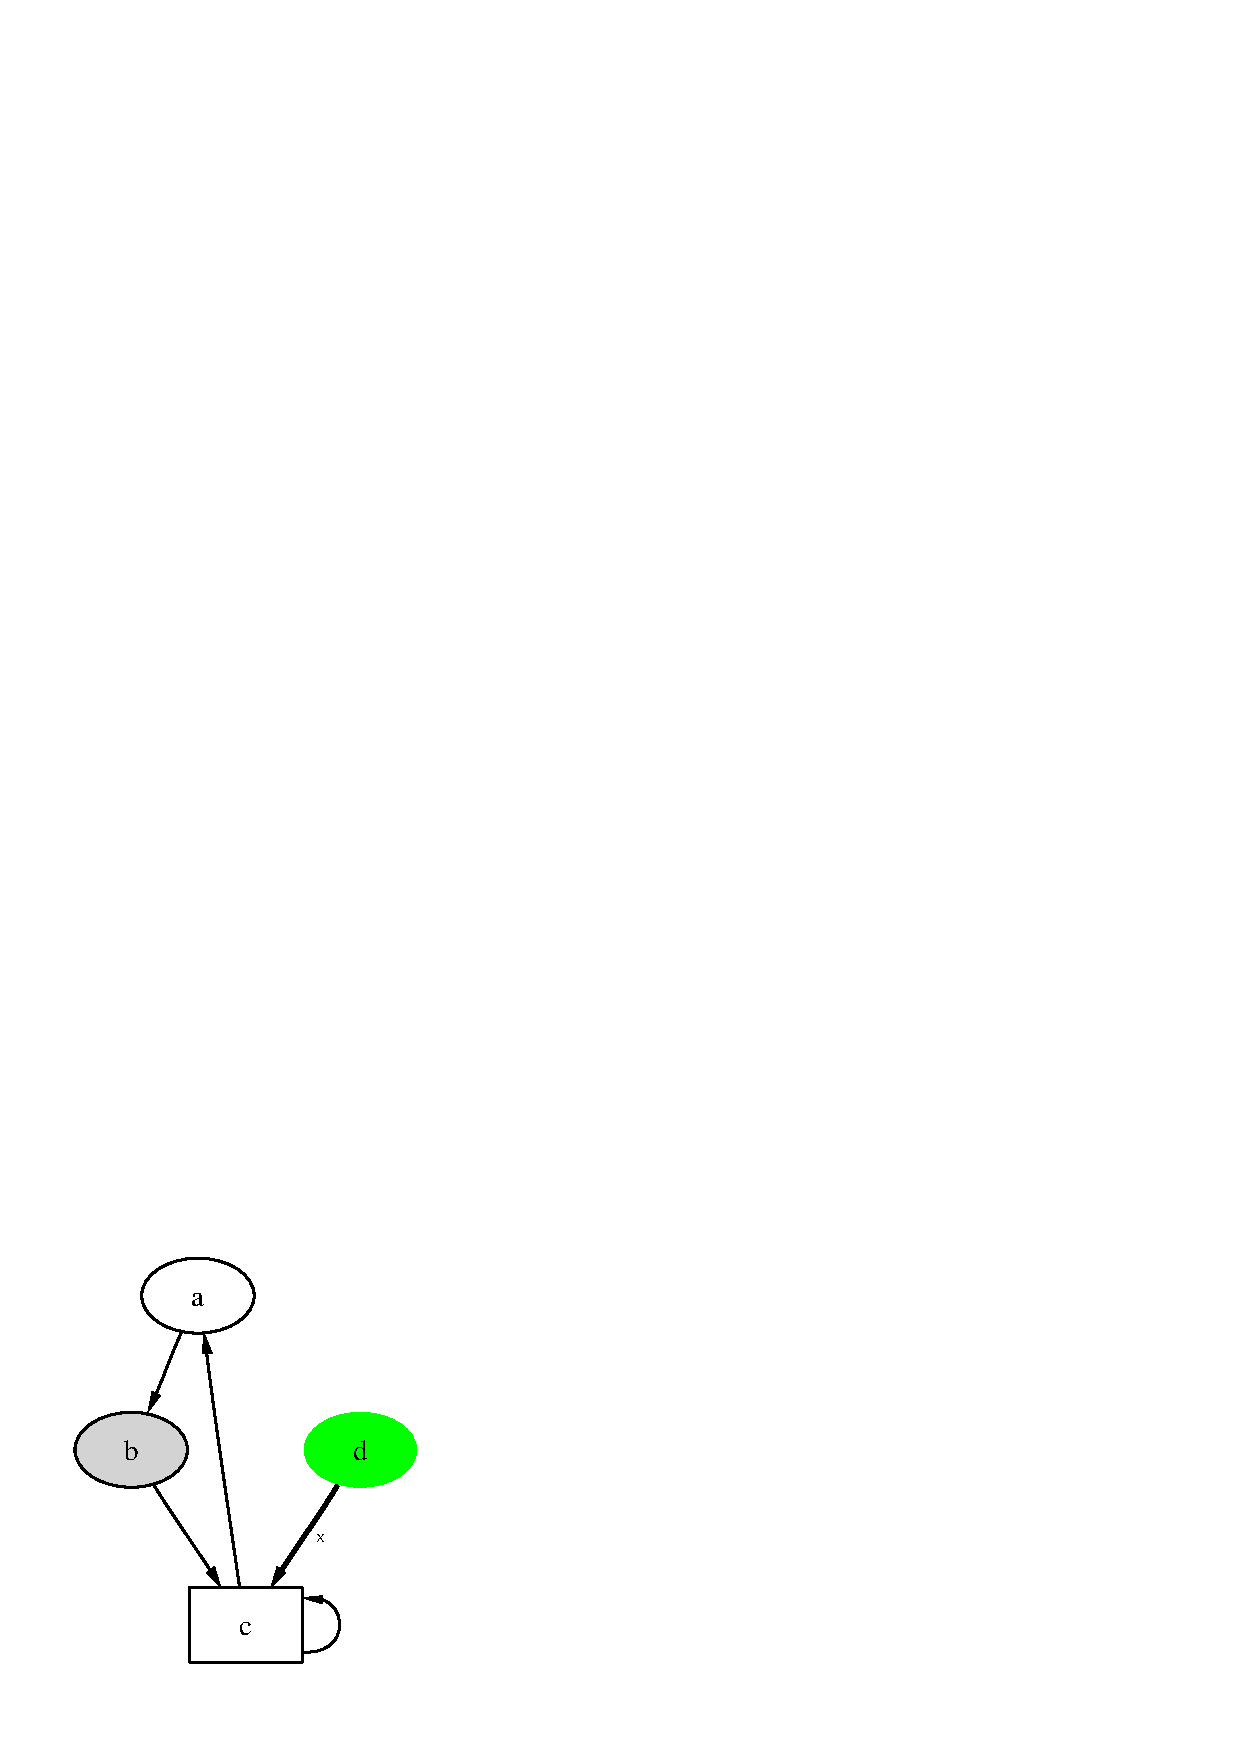
\epsfig{file = example.pdf, width = 4.5cm}
\end{center}
\caption{Un grafo generato con dot.}\label{fig:dot_example}
\end{figure}
%
Il linguaggio dot (\texttt{http://www.graphviz.org/}) permette di
disegnare grafi a partire da una loro specifica testuale data in
termini di nodi e archi fra nodi. Si consideri per esempio il grafo
in Figura~\ref{fig:dot_example}. Esso \`e stato generato a partire dal
seguente file sorgente \texttt{example.dot}, scritto nel linguaggio dot:
%
\begin{verbatim}
  digraph example {
    size = "11,7.5"

    a [label = "a"]
    b [label = "b" style = filled]
    c [label = "c" shape = box]
    d [label = "d" color = green style = filled]

    a -> b
    b -> c
    c -> c
    c -> a
    d -> c [label = "X" fontsize = 6 style = bold]
  }
\end{verbatim}
%
In tale sorgente si specificano, in un qualsiasi ordine, i nodi e
gli archi del grafo. Nodi e archi possono avere propriet\`a espresse fra
parentesi quadre per specificarne la forma, lo spessore o il colore.
La trasformazione di tale file sorgente nel file postscript in
Figura~\ref{fig:dot_example} avviene tramite il comando:
%
\begin{verbatim}
  dot -Tps example.dot >example.ps
\end{verbatim}
%
Ulteriori esempi sono presenti nella pagina web di dot.
\`E possibile avere ulteriori informazioni su dot anche tramite
il manuale in linea: \texttt{man dot}.

Adesso che abbiamo capito come si specifica un grafo tramite il linguaggio
dot, poniamoci il problema di generare un file sorgente dot a partire da una
classe di sintassi astratta che descrive una parte di codice Kitten.
Per esempio, la sintassi concreta
\texttt{!this.state} in Figura~\ref{fig:led} \`e tradotta nel sottoalbero
di sintassi astratta radicato in \texttt{Not} in Figura~\ref{fig:led_albero}.
Tale sottoalbero \`e specificato da un file sorgente dot del tipo:
%
\begin{verbatim}
  node19 [label = "Not"]
  node18 [label = "FieldAccess"]
  node17 [label = "Variable"]
  symbol_this [label = "this" fontname = "Times-Italic" shape = box]
  node17 -> symbol_this [label = "name" fontsize = 8]
  node18 -> node17 [label = "receiver" fontsize = 8]
  symbol_state [label = "state" fontname = "Times-Italic" shape = box]
  node18 -> symbol_state [label = "name" fontsize = 8]
  node19 -> node18 [label = "expression" fontsize = 8]
\end{verbatim}
%
Si noti che l'esatta numerazione dei nodi non \`e importante, a differenza
della loro etichetta che apparir\`a nel file postscript finale.
Quello che importa per\`o \`e che tale numerazione generi stringhe diverse
per nodi di sintassi astratta diversi, anche se poi la loro etichetta esterna,
quella visualizzata nel file postscript,
pu\`o coincidere. A tal fine, basta che ogni nodo di sintassi
astratta contribuisca al file dot con un nodo chiamato \texttt{node}$n$,
dove $n$ \`e l'identificatore unico di tale nodo (si veda il campo
\texttt{identifier} in Figura~\ref{fig:absyn.Absyn}). I simboli sono
invece condivisi e mai ripetuti (Figura~\ref{fig:symbol.Symbol}).
Essi saranno quindi rappresentati da un nodo chiamato \texttt{symbol\_}$x$,
dove $x$ \`e l'identificatore del simbolo.

La generazione del file sorgente dot \`e fatta con un algoritmo
a discesa ricorsiva:
un nodo di sintassi astratta genera una parte del file
che descrive se stesso e gli archi verso i suoi figli; quindi chiama
ricorsivamente la generazione della parte di file per i suoi figli.
Per esempio, il file precedente viene generato in questo modo:
il nodo \texttt{Not} genera le righe
%
\begin{verbatim}
  node19 [label = "Not"];
  node19 -> node18 [label = "expression" fontsize = 8]
\end{verbatim}
%
Quindi il nodo figlio di \texttt{Not}, \cioe un \texttt{FieldAccess},
genera le righe
%
\begin{verbatim}
  node18 [label = "FieldAccess"];
  node18 -> node17 [label = "receiver" fontsize = 8]
  node18 -> symbol_state [label = "name" fontsize = 8]
\end{verbatim}
%
I due nodi figli di \texttt{FieldAccess} sono una \texttt{Variable}, che
genera
%
\begin{verbatim}
  node17 [label = "Variable"];
  node17 -> symbol_this [label = "name" fontsize = 8]
\end{verbatim}
%
e un \texttt{Symbol}, che genera
%
\begin{verbatim}
  symbol_state [label = "state" fontname = "Times-Italic" shape = box]
\end{verbatim}
%
Infine, il figlio di \texttt{Variable} \`e un \texttt{Symbol} che genera
%
\begin{verbatim}
  symbol_this [label = "this" fontname = "Times-Italic" shape = box]
\end{verbatim}

Sebbene sia possibile dare una definizione formale della generazione
del file dot, limitiamoci per semplicit\`a a mostrarne l'implementazione Java.
Per prima cosa, aggiungiamo alcuni metodi di utilit\`a alla classe
\texttt{absyn/Absyn.java}. Questi sono mostrati in
Figura~\ref{fig:absyn.Absyn_dot}.
\begin{itemize}
\item Il metodo \texttt{label()} restituisce
l'etichetta che deve essere visualizzata dentro il nodo dot che
rappresenta un nodo di sintassi astratta. Normalmente, si tratta del
nome della classe di sintassi astratta, senza il prefisso che indica il
package \texttt{absyn} (per questo si usa \texttt{getSimpleName()}
piuttosto che \texttt{getName()}). Si noti che le sottoclassi potrebbero
ridefinire questo metodo. Per esempio, le classi per i letterali
ridefiniscono questo metodo in modo da specificare anche il valore lessicale
del letterale.
\item Il metodo \texttt{dotNodeName()} restituisce il nome usato nel file dot
per fare riferimento a un nodo di sintassi astratta. Come detto, si tratta
della stringa \texttt{node}$n$ dove $n$ \`e l'identificatore unico del
nodo di sintassi astratta.
\item Il metodo \texttt{linkToNode()} scrive dentro un file testo il comando
dot che crea un arco fra il nodo \texttt{this} di sintassi astratta e un
nodo di sintassi astratta il cui nome usato nel file dot \`e \texttt{to}.
Occorre anche specificare l'etichetta \texttt{name} dell'arco.
\item Il metodo \texttt{boldLinkToNode()} si comporta come
\texttt{linkToNode()} ma crea un arco di maggiore spessore. Questo
metodo \`e usato solo per legare un comando o un membro di una classe
al suo successore (campi \texttt{next}). Si veda per esempio la
Figura~\ref{fig:led_albero}.
\end{itemize}
%
\begin{figure}[t]
\begin{verbatim}
protected String label() {
  return this.getClass().getSimpleName();
}

protected final String dotNodeName() {
  return "node" + identifier;
}

protected final void linkToNode(String name, String to, FileWriter where)
{
  where.write(dotNodeName() + " -> " + to +
              " [label = \"" + name + "\" fontsize = 8]\n");
}

protected final void boldLinkToNode
  (String name, String to, FileWriter where)
{
  where.write(dotNodeName() + " -> " + to +
              " [label = \"" + name + "\" fontsize = 8 style = bold]\n");
}
\end{verbatim}
\caption{Metodi aggiunti alla classe \texttt{absyn/Absyn.java} in Figura~\ref{fig:absyn.Absyn} per la generazione della rappresentazione dot della sintassi astratta.}
  \label{fig:absyn.Absyn_dot}
\end{figure}

A questo punto possiamo definire un metodo ricorsivo per la generazione del
file dot a partire da un nodo di sintassi astratta. Lo chiameremo
\texttt{toDot()}. La sua intestazione \`e:
%
\begin{verbatim}
  public String toDot(FileWriter where)
\end{verbatim}
%
Questo significa che il metodo scrive dentro il file indicato il codice
dot che rappresenta la classe di sintassi astratta e i suoi figli (e
ricorsivamente i figli dei figli\ldots). Il valore
di ritorno \`e il nome usato nel file dot per rappresentare il nodo
di sintassi astratta su cui il metodo \`e invocato.

Cominciamo dai tipi. Il metodo \texttt{toDot()} \`e \cosi definito in
\texttt{absyn/TypeExpression.java}:
%
\begin{verbatim}
  public final String toDot(FileWriter where) {
    where.write(dotNodeName() + " [ label = \"" + label() + "\"];\n");
    toDot$0(where);
    return dotNodeName();
  }

  protected void toDot$0(FileWriter where) {}
\end{verbatim}
%
Si noti che \texttt{toDot()}
\`e definito come \texttt{final}. Esso si limita a generare
un nodo dot per il nodo di sintassi astratta e a chiamare un metodo ausiliario
\texttt{protected} che di default non fa nulla. Le ridefinizioni del
metodo \texttt{toDot\$0()} creano degli archi
verso i nodi figli e richiamano ricorsivamente \texttt{toDot()}.
Per esempio, eccone la ridefinizione dentro
\texttt{absyn/ArrayTypeExpression.java}:
%
\begin{verbatim}
  protected void toDot$0(FileWriter where) {
    linkToNode("elementsType",elementsType.toDot(where),where);
  }
\end{verbatim}
%$

Lo stesso procedimento si usa per le espressioni.
La definizione di \texttt{toDot()} dentro alla classe
\texttt{absyn/Expression.java} \`e
identica al caso dei tipi. La ridefinizione di \texttt{toDot\$()} dentro
\texttt{absyn/Variable.java} \`e per esempio
%
\begin{verbatim}
  protected void toDot$0(FileWriter where) {
    linkToNode("name",name.toDot(where),where);
  }
\end{verbatim}
%$
e quella dentro \texttt{absyn/FieldAccess.java} \`e:
%
\begin{verbatim}
  protected void toDot$0(FileWriter where) {
    linkToNode("receiver",receiver.toDot(where),where);
    linkToNode("name",name.toDot(where),where);
  }
\end{verbatim}
%$
Come altro esempio, la ridefinizione di \texttt{toDot\$0()} dentro
\texttt{absyn/BinOp.java} \`e
%
\begin{verbatim}
  protected void toDot$0(FileWriter where) {
    linkToNode("left",left.toDot(where),where);
    linkToNode("right",right.toDot(where),where);
  }
\end{verbatim}
%$

Vediamo infine la definizione di \texttt{toDot()} dentro
\texttt{symbol/Symbol.java} (Figura~\ref{fig:symbol.Symbol}):
%
\begin{verbatim}
  public String toDot(FileWriter where) {
    where.write("symbol_" + name +
                " [label = \"" + name + "\"" +
                " fontname = \"Times-Italic\" shape = box]\n");
    return "symbol_" + name;
  }
\end{verbatim}
%
Questa volta il metodo genera un nodo dot di nome \texttt{symbol\_}$x$,
dove $x$ \`e il nome del simbolo. I simboli non hanno mai archi uscenti, per
cui costituiscono un caso base della discesa ricorsiva (le foglie
dell'albero in Figura~\ref{fig:led_albero}).

La definizione di \texttt{toDot()} \`e simile per i comandi. Per la
struttura complessiva di una classe, il metodo \texttt{toDot()}
si richiama ricorsivamente sui componenti della classe e aggiunge al file
dot un prologo che specifica la dimensione della pagina e un epilogo, \cioe
la parentesi graffa di chiusura!
%
\javatip{
L'aggiunta di una nuova classe di sintassi astratta al compilatore
Kitten comporta
la definizione del suo metodo \texttt{toDot\$0()}. Come visto in questi
esempi, si tratta semplicemente di una sequenza di
chiamate a \texttt{linkToNode()} per ciascuno dei figli della classe
di sintassi astratta che \`e stata aggiunta. In assenza della specifica
del metodo
\texttt{toDot\$0()}, il comportamento di default sar\`a quello dell'omonimo
metodo, vuoto, definito in \texttt{absyn/TypeExpression.java} per i tipi,
\texttt{absyn/Expression.java} per le espressioni e
\texttt{absyn/Command.java} per i comandi. Conseguentemente non sar\`a
visibile, nel file postscript generato da dot, il sottoalbero
radicato nei nodi di sintassi astratta per la nuova classe che \`e
stata aggiunta. Un comportamento indesiderato che non finisce
di meravigliare gli studenti\ldots}
%
\begin{exercise}\label{ex:descent_fields}
Si formalizzi uno schema a discesa ricorsiva che calcola l'insieme dei
nomi di campi letti in un comando. Si faccia lo stesso per l'insieme
dei nomi delle classi istanziate in un comando.
\end{exercise}
%
\begin{exercise}\label{ex:expressions_simplify}
Si definisca con una discesa ricorsiva un giudizio
$\vdash^{\mathsf{simp}}$ tale che
$\mathit{exp}\vdash^{\mathsf{simp}}\mathit{exp}'$ \`e vero quando
l'espressione Kitten $\mathit{exp}'$ \`e ottenuta \emph{semplificando}
un'altra espressione Kitten $\mathit{exp}$. La semplificazione da considerare
\`e quella che sostituisce operazioni binarie fra costanti numeriche
con il loro risultato. Una costante numerica \`e un letterale numerico
o un'operazione binaria aritmetica fra costanti numeriche.
Si schematizzi quindi l'implementazione Java di $\vdash^{\mathsf{simpl}}$.
Riportiamo sotto alcuni esempi di coppie $\mathit{exp}$ ed $\mathit{exp}'$:
%
\[
{\scriptsize
\begin{array}{|c|c|}\hline
  \mathit{exp} & \mathit{exp'}\\\hline\hline
  \mathtt{Addition(IntLiteral(4),IntLiteral(5))} & \mathtt{IntLiteral(9)} \\
    \hline
  \mathtt{LessThan(IntLiteral(4),IntLiteral(5))} & \mathtt{True()} \\\hline
  \mathtt{Addition(Multiplication(IntLiteral(4),IntLiteral(5)),
    Variable(x))} & \mathtt{Addition(IntLiteral(20),Variable(x))}\\\hline
\end{array}
}
\]
\end{exercise}
